%
% section 2.1
%
% \setcounter{section}{0}
\section{Φυσικό Επίπεδο - Επίπεδο Σύνδεσης (Ζεύξης) Δεδομένων (Μοντέλο OSI)}

Το χαμηλότερο επίπεδο στο OSI, όπως έχουμε ήδη αναφέρει, είναι το \emph{φυσικό}. Το επίπεδο αυτό είναι υπεύθυνο για τη μετάδοση των bits μέσα από το ενσύρματο ή ασύρματο τηλεπικοινωνιακό κανάλι. Το φυσικό επίπεδο καθορίζει τα ηλεκτρικά και μηχανικά χαρακτηριστικά της σύνδεσης του σταθμού με το μέσο μετάδοσης.

\emph{Τα μηχανικά χαρακτηριστικά} καθορίζουν λεπτομέρειες όπως το  είδος του συνδέτη (βύσματος) του δικτύου, τις διαστάσεις του, τις ανοχές, το πλήθος των ακροδεκτών, τον τρόπο με τον οποίο ασφαλίζει πάνω στο δικτυακό εξοπλισμό κλπ. Τα \emph{ηλεκτρικά χαρακτηριστικά} καθορίζουν τον τρόπο με τον οποίο αναπαρίστανται τα bit 0 και 1 στο φυσικό μέσο (π.χ. τα επίπεδο τάσης σε ένα ενσύρματο δίκτυο που αναπαριστούν σε ηλεκτρικό σήμα τα 0 και 1). Στο φυσικό επίπεδο επίσης καθορίζεται αν η μετάδοση μπορεί να γίνει μόνο προς μια μεριά (half duplex) ή και προς τις δύο (full duplex) ταυτόχρονα. Το φυσικό επίπεδο δεν ενδιαφέρεται αν αυτό που μεταφέρει είναι bytes (8bits) ή χαρακτήρες ASCII των 7bits. 

\begin{inthebox}
\textbf{Τι είναι το ASCII; Υπάρχει 7bit ASCII;}

Το ASCII είναι ίσως από τα πλέον παλιά, κοινά αποδεκτά πρότυπα των υπολογιστών. Προέρχεται από τα αρχικά των λέξεων American Standard Code for Information Interchange και είναι ένας κώδικας που αντιστοιχεί κάθε γράμμα του λατινικού αλφαβήτου σε ένα αριθμό. Έτσι για παράδειγμα το A αντιστοιχεί στο 65, το B στο 66 κ.ο.κ. Εκτός από τα γράμματα κωδικοποιούνται αντίστοιχα τα ψηφία από 0 ως 9 και διάφορα σύμβολα. Για παράδειγμα το θαυμαστικό (!) είναι το 33, τα εισαγωγικά το 34 και το κενό διάστημα το 32. Οι χαρακτήρες από 0-31 δεν χρησιμοποιούνται για κανονικά γράμματα ή σύμβολα αλλά περιέχουν χαρακτήρες ελέγχου. Αυτοί όταν εκτυπώνονται εκτελούν κάποια ειδική λειτουργία ανάλογα με το τερματικό που χρησιμοποιείται. Π.χ. ο χαρακτήρας 7 στέλνει ηχητικό σήμα στο μεγαφωνάκι του τερματικού (ονομάζεται  BEL(L) για ιστορικούς λόγους, που θα σας αναφέρω στο μάθημα!). Άλλοι ειδικοί χαρακτήρες μπορεί π.χ. να μετακινούν το δρομέα πάνω στην οθόνη κ.λ.π.

Αν χρησιμοποιήσουμε 7bit για το ASCII, μπορούμε να έχουμε ως 128 χαρακτήρες. Στις περισσότερες περιπτώσεις χρησιμοποιούμε 8bit ASCII (256 χαρακτήρες) που είναι απαραίτητο για να βάλουμε επιπλέον αλφάβητο εκτός από το λατινικό.

Φυσικά στις μέρες μας τίποτα από τα δύο δεν αρκεί, καθώς στο Internet χρειαζόμαστε ταυτόχρονα πολύ περισσότερους χαρακτήρες από ότι προσφέρει το ASCII. Η ανάγκη αυτή καλύπτεται με τεχνολογίες όπως το unicode.\\
\end{inthebox}

\begin{figure}[!ht]
  \centering
  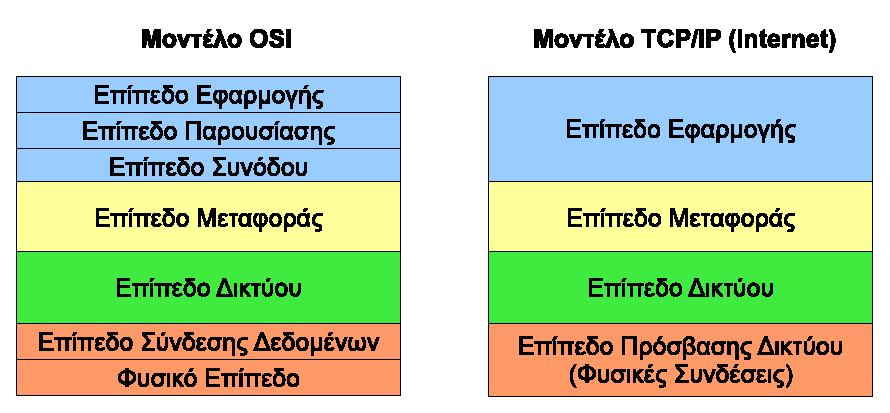
\includegraphics[width=0.95\textwidth]{images/chapter2/2-1}
  \caption {\textsl{Μοντέλα OSI και TCP/IP}}
  \label{2-1}
\end{figure}

Ακριβώς πάνω από το φυσικό επίπεδο του OSI, βρίσκεται το \emph{επίπεδο σύνδεσης (ζεύξης) δεδομένων - Data Link Layer}. Το επίπεδο αυτό έχει σκοπό να κάνει αξιόπιστη τη φυσική γραμμή σύνδεσης μεταξύ δύο σταθμών. Το επίπεδο αυτό λαμβάνει τα δεδομένα του από το πιο πάνω επίπεδο (επίπεδο δικτύου) με τη μορφή πακέτων. Από αυτά τα πακέτα δημιουργεί πλαίσια δεδομένων.  Το επίπεδο σύνδεσης δεδομένων:

\begin{itemize}
\item Δημιουργεί πλαίσια δεδομένων από τα πακέτα που λαμβάνει. Σε κάθε πλαίσιο προσθέτει κατάλληλη επικεφαλίδα (header) και ουρά (trailer)
\item Ανιχνεύει τα σφάλματα μετάδοσης και είτε τα διορθώνει είτε ζητά την επανεκπομπή τους
\item Ελέγχει πότε μπορεί να δεσμεύσει το φυσικό μέσο ώστε να ξεκινήσει την αποστολή των πλαισίων χωρίς κίνδυνο σύγκρουσης με άλλο σταθμό
\item Μεταβάλλει την ροή των πλαισίων ανάλογα με τους ρυθμούς που μπορεί να δεχθεί ο παραλήπτης
\end{itemize}

Όπως έχουμε ήδη αναφέρει, το κατώτερο επίπεδο στο TCP/IP είναι το πρόσβασης δικτύου το οποίο αντιστοιχεί στα δύο επίπεδα του OSI που περιγράψαμε παραπάνω (σχήμα \ref{2-1}). Το επίπεδο πρόσβασης δικτύου παρέχει την πρόσβαση στο φυσικό μέσο στο οποίο η πληροφορία μεταδίδεται με μορφή πακέτων και αντιπροσωπεύει το χαμηλότερο επίπεδο λειτουργικότητας που απαιτείται από ένα δίκτυο. Το επίπεδο αυτό περιλαμβάνει όλα τα στοιχεία των φυσικών συνδέσεων (καλώδια, αναμεταδότες, κάρτες δικτύου, πρωτόκολλα πρόσβασης τοπικών δικτύων) και προσφέρει τις υπηρεσίες του στο επίπεδο δικτύου. Το TCP/IP δεν καθορίζει τον ακριβή τρόπο λειτουργίας του επιπέδου αυτού, αφού απλά προδιαγράφει ότι πρέπει να είναι ικανό να μεταδίδει με κάποιο τρόπο τα δεδομένα που λαμβάνει σε μορφή πακέτων από το επίπεδο δικτύου. Στο επίπεδο αυτό μπορούν να χρησιμοποιούνται διαφορετικές τεχνολογίες και οι λεπτομέρειες τους καθορίζονται από τους κατασκευαστές των δικτύων και των αντίστοιχων συσκευών.